\documentclass{standalone}
\usepackage{tikz}
\usetikzlibrary{positioning, fit, shapes, arrows}



\pgfdeclarelayer{bg}    % declare background layer
\pgfsetlayers{bg,main}  % set the order of the layers (main is the standard layer)

%% from https://tex.stackexchange.com/questions/356564/macro-for-rounded-polygon-around-some-nodes
%% answer of bitt.j
%Necessary for the mypoly command%
\usepackage{tkz-euclide}
\usepackage{xstring}

%------------------------%
%---The mypoly command---%
%------------------------%

%--Getting the last Element of a list--%
\def\splicelist#1{
\StrCount{#1}{,}[\numofelem]
\ifnum\numofelem>0\relax
     \StrBehind[\numofelem]{#1}{,}[\mylast]%
\else
    \let\mylast#1%
\fi
}

%--The mypoly macro--%
%How to use:
%\myroundpoly[decorative commands]{list of names of nodes}{distance}
%list of names has to be given in clockwise order
\newcommand{\hedge}[3][thin,color=black]{
%Get the last element
\splicelist{#2}
%Calculate the auxiliary coordinates for the arcs
\foreach \vertex [remember=\vertex as \succvertex
    (initially \mylast)] in {#2}{
    \coordinate (\succvertex-next) at ($(\succvertex)!#3!90:(\vertex)$);
    \coordinate (\vertex-previous) at ($(\vertex)!#3!-90:(\succvertex)$);
    \draw[#1] (\succvertex-next) --  (\vertex-previous);
}
%Draw the arcs
\foreach \vertex in {#2}{
    \tkzDrawArc[#1](\vertex,\vertex-next)(\vertex-previous)
}
}



\begin{document}
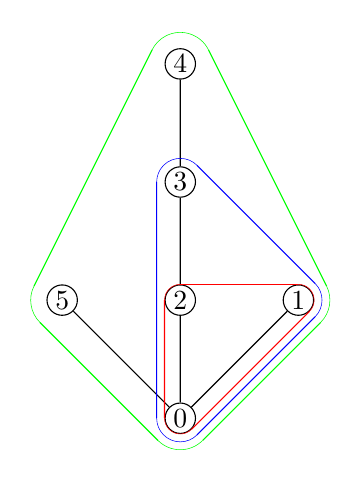
\begin{tikzpicture}[every node/.style={draw, circle, inner sep=1pt}, grow=up]
\node(0) {0}
   child{node(1){1}}
   child{node(2){2}
       child{node(3){3}
       child{node(4){4}}
       }}
   child{node(5){5}};
% \begin{pgfonlayer}{bg}    % select the background layer
\hedge[red]{0,2,1}{0.2cm}
\hedge[blue]{0,2,3,1}{0.3cm}
\hedge[green]{0,5,4,1}{0.4cm}
%\end{pgfonlayer}
\end{tikzpicture}
\end{document}
